
%%%%%%%%%%%%%%%%%%%%%%%%%%%%%%%%%%%%%%%%%
% University/School Laboratory Report
% LaTeX Template
% Version 3.1 (25/3/14)
%
% This template has been downloaded from:
% http:\\www.LaTeXTemplates.com
%
% Original author:
% Linux and Unix Users Group at Virginia Tech Wiki 
% (https:\\vtluug.org/wiki/Example_LaTeX_chem_lab_report)
%
% License:
% CC BY-NC-SA 3.0 (http:\\creativecommons.org/licenses/by-nc-sa/3.0/)
%
%%%%%%%%%%%%%%%%%%%%%%%%%%%%%%%%%%%%%%%%%

%----------------------------------------------------------------------------------------
%	PACKAGES AND DOCUMENT CONFIGURATIONS
%----------------------------------------------------------------------------------------

\documentclass[12pt]{article}
\usepackage{booktabs}
\usepackage{float}
\usepackage{fontspec}
\usepackage{mathtools}
\usepackage{xcolor}
\usepackage{titlesec}
%\usepackage{arial}
\usepackage{mathptmx}
\usepackage[version=3]{mhchem} % Package for chemical equation typesetting
\usepackage{siunitx} % Provides the \SI{}{} and \si{} command for typesetting SI units
\usepackage{graphicx} % Required for the inclusion of images
\usepackage{hyperref}
\usepackage{amsmath} % Required for some math elements 
\usepackage{inputenc}
\usepackage[T1]{fontenc}
%\usepackage[portuguese]{babel}
% \usepackage{hyphenat}
\usepackage{helvet}
\usepackage{titlesec}
\usepackage{titling}
\usepackage{setspace}
\usepackage{booktabs}
\usepackage[acronym,nomain,nonumberlist,toc]{glossaries} % 
\usepackage[british,UKenglish,USenglish,american]{babel}

%\hyphenation{mate-mática recu-perar}

\usepackage{etoolbox}

\AtBeginDocument{%
	\setlength{\abovedisplayskip}{6pt}
	\setlength{\belowdisplayskip}{6pt}
}

\setcounter{tocdepth}{6}
\setcounter{secnumdepth}{6}



\makeatletter
\g@addto@macro\normalsize{%
	\setlength\abovedisplayskip{6pt}
	\setlength\belowdisplayskip{6pt}
	\setlength\abovedisplayshortskip{6pt}
	\setlength\belowdisplayshortskip{6pt}
}
\makeatother

\setlength\parindent{0pt} % Removes all indentation from paragraphs

\renewcommand{\labelenumi}{\alph{enumi}.} % Make numbering in the enumerate environment by letter rather than number (e.g. section 6)

\setsansfont{Arial}
% Set serifed font to Cambria
%\setmainfont{Times New Roman}
\setmainfont[SizeFeatures={Size=12}]{Arial}
\newfontfamily\subsubsectionfont{Times New Roman} %12pt large
\newfontfamily\headingfont[]{Arial}
% Set formats for each heading level
\titleformat*{\section}{\Large\bfseries\sffamily}
\titleformat*{\subsection}{\Large\bfseries\sffamily}
\titleformat*{\subsubsection}{\itshape\subsubsectionfont}

\font\myfon=Arial at 17pt
\font\myfont=Arial at 15pt
\font\myfontt=Arial at 12pt

\usepackage{enumitem}
\usepackage{booktabs}
\usepackage{graphicx}


\newfontfamily\capfont[SizeFeatures={Size=10}]{Times New Roman}
\newfontfamily\mathfont[SizeFeatures={Size=12}]{Times New Roman}


\usepackage{caption}
\DeclareCaptionFont{cap}{\capfont}

\makeatletter %only needed in preamble
\renewcommand\scriptsize{\@setfontsize\scriptsize{10pt}{10pt}}
\makeatother
\captionsetup{font=cap, labelfont=cap}

\usepackage{subcaption}
\usepackage{wrapfig}

\renewcommand{\thesection}{\Roman{section}.} 
\renewcommand{\thesubsection}{\thesection\Roman{subsection}}
\renewcommand{\baselinestretch}{1.5} 

\titlespacing*{\section}
{0pt}{6pt}{3pt}

\titlespacing*{\subsection}
{0pt}{6pt}{3pt}

\titlespacing*{\subsubsection}
{0pt}{6pt}{3pt}

%\setmainfont{mathptmx}

\usepackage{geometry}
\geometry{
	a4paper,
	total={170mm,257mm},
	left=20mm,
	top=20mm,
}


\usepackage{spverbatim}


\usepackage{listings}
\lstset{
	keywordstyle=\color{RoyalBlue},
	basicstyle=\small\ttfamily,
	commentstyle=\color{black}\ttfamily,
	%    rulecolor=\color{black},
	showstringspaces=false,
	breaklines=true,
	frameround=ftff,
	frame=single,
	columns=flexible,
	%    belowcaptionskip=5em,
	aboveskip=1.25em,
	language=Verilog,
}

\renewcommand{\lstlistingname}{Code excerpt} 

 \setlength{\belowcaptionskip}{-10pt}





\begin{document}
	
	
	%----------------------------------------------------------------------------------------------------------------------------------------------------------------------------------------------------
	%																					CAPA
	%----------------------------------------------------------------------------------------------------------------------------------------------------------------------------------------------------
	
	%----------------------------------------------------------------------------------------------------------------------------------------------------------------------------------------------------
	%----------------------------------------------------------------------------------------------------------------------------------------------------------------------------------------------------
	\begin{titlepage}
		\begin{figure}
			
\includegraphics[scale=0.4]{IST} 
		\end{figure}
		
		\vspace*{3cm}
		\begin{center}
			\headingfont\Large{\bfseries INSTITUTO SUPERIOR TÉCNICO}\\[2cm]
			\headingfont\LARGE{\bfseries Design Test and Reliability of Electronic Systems \\[1,5cm]Project 2 - Circular Bist}\\[0,5cm]
			%\headingfont\Large{\bfseries RELATÓRIO FORMAL}
		\end{center}
		\vspace{3cm}
		\headingfont\hfill
		\begin{tabular}{@{}l@{}}
		    Group 2\\ 
			n$^{\circ}$ 77973 - Pedro Pina\\
			n$^{\circ}$ 84779 - Afonso Muralha\\
			\\
			Professor Fernando Gonçalves
			
		\end{tabular}
		\vspace{2,5cm}
		\begin{center}
			\today
		\end{center}
	\end{titlepage}
	%----------------------------------------------------------------------------------------------------------------------------------------------------------------------------------------------------
	%																						CAPA
	%----------------------------------------------------------------------------------------------------------------------------------------------------------------------------------------------------
	\newpage

    \tableofcontents

	\newpage



	\section{Introduction and Objectives}
	The goal of this second project of the Design Test and Reliability of Electronic Systems course is to implement a Circular built-in self-test (BIST) system to circuit assigned.\\
	The developed system must be submitted to a fault simulator that will inject faults on the top module of the system an will check for fault detection. The fault coverage must be higher than 90\%.
	
	\section{Circular BIST design}
	The circular BIST system must be applied to a given circuit, different for each group. The circuit in question is named ''circuito06'' and its as follows: 
	\begin{figure}[!htb]
        \centering
        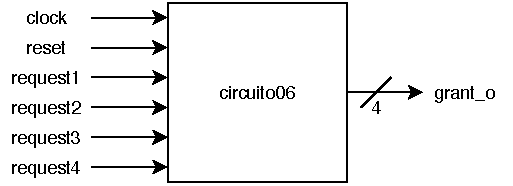
\includegraphics[scale=1]{circuito06.pdf}
            \caption{''circuito06'' interface.}
            \label{fig:ci}
    \end{figure}
    
    In order to make it compatible with the BIST scan chain, scan functionality needed to be added. This was done using cadence tools and it added the ''scan\textunderscore in'' and ''mode'' inputs and the ''scan\textunderscore out'' output.
    
    
    
    \subsection*{LFSR and MISR}
    
    In order to generate pseudo-random inputs for the circuit, an external linear feedback shift register (LFSR) is implemented. 
    
    \begin{figure}[!htb]
        \centering
        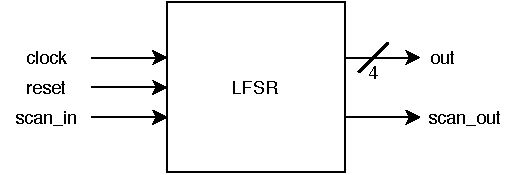
\includegraphics[scale=1]{images/LFSR.pdf}
            \caption{LFSR block diagram.}
            \label{fig:lfsrbd}
    \end{figure}
    
    Since there are 4 inputs for the circuit, the LFSR features 4 flip-flop stages with XOR feedback on the forth and third flip-flops in order to make the output polynomial maximal-length:
    
    \begin{equation}
        \begin{matrix}
            \text{Polynomial} = x^{4} + x^{3} + 1 
            \\ 
            \text{Period}= 2^{4} -1 = 15
        \end{matrix}
    \end{equation}
    
    Finally, to make it scan compatible, the scan\textunderscore in was added to the XOR chain and a scan\textunderscore out port using the last flip-flop state was added. This adds another degree of randomness to the system and makes it more likely for the system to detect faults.
    Additionally a temporary seed input was added for testing purposes.
    
    The LFSR is represented in verilog:
  
    \begin{lstlisting}[caption={LFSR code.},captionpos=b]
module lfsr #
(   
    parameter NBIT = 4,
    parameter SEED = 4'b1111
) (
    input clk,
    input rst,
    input scan_in,
    // input [3:0] seed, //this is only used for testing
    output [NBIT-1:0] out,
    output scan_out
);

    reg [NBIT-1:0] dff;

    assign out[0] = dff[0];
    assign out[1] = dff[1];
    assign out[2] = dff[2];
    assign out[3] = dff[3];
    
    assign scan_out = dff[3];

    always @ (posedge clk) begin
        if(rst) begin
            dff <= SEED;
        end
        else begin
            dff <= {dff[4-2:0], dff[3] ^ dff[2] ^ scan_in};
        end
    end

endmodule
    \end{lstlisting}
    
    A test-bench was created to ensure the periodicity of the LFSR. The test-bench is able to set a user determined seed and will cycle the LFSR until the output patterns repeats. When it does, the iteration number is printed and the program execution stops. In this case, the scan input is disabled. Since the LFSR has 4 bits, the number of cycles until repetition should be $2^{N}-1 = 2^{4}-1= 15$\\
    Test result:
        
        \begin{lstlisting}[caption={LFSR test-bench.},captionpos=b]
linuxdev@linuxdev-VirtualBox:/media/sf_GitHub/PTFSE-Classes/Project2$ make lfsr_test
Initial seed:          15
LFSR output: 15
LFSR output: 14
LFSR output: 12
LFSR output:  8
LFSR output:  1
LFSR output:  2
LFSR output:  4
LFSR output:  9
LFSR output:  3
LFSR output:  6
LFSR output: 13
LFSR output: 10
LFSR output:  5
LFSR output: 11
LFSR output:  7
End in          15 iterations
Should be 2^4-1 =          15
    \end{lstlisting}

With this, we can assure that the LFSR is working and can be used on the top module.\\
\newpage
    
In order to register the output combinations of the circuit, an internal multiple input signature register is also created. 

\begin{figure}[!htb]
        \centering
        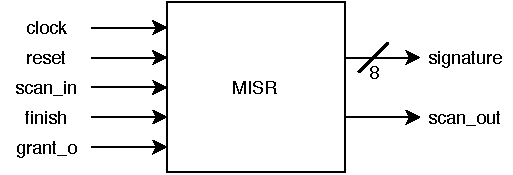
\includegraphics[scale=1]{images/MISR.pdf}
            \caption{MISR block diagram.}
            \label{fig:misrbd}
    \end{figure}

With this the input sequence of the MISR will generate a quasi-unique signature for a BIST run. The length chosen for the MISR was 8, but other sizes were tested, for example, 16, but since it did not improve the fault coverage, the size was reset to 8, since more hardware can be worst for the fault coverage. With 8 flip-flops the XOR chain used in order to make output polynomial maximal-length was:
    
    \begin{equation}
            \text{Polynomial} = x^{8} + x^{6} + x^{5} + x^{4} + 1 
    \end{equation}   

An additional input named ''finish'' was added. This serves the purpose of holding the final signature. This input is controlled by the ''finish'' output of the controller.
The MISR is represented in verilog:
  
    \begin{lstlisting}[caption={MISR code.},captionpos=b]
// `define misr16
`define misr8

module misr #
(
    `ifdef misr16
    parameter NBIT = 16
    `endif

    `ifdef misr8
    parameter NBIT = 8
    `endif
)(
    input clk,
    input rst,
    input scan_in,
    input[3:0] grant_o,
    input finish,
    output[NBIT-1:0] signature,
    output scan_out
);

    reg [NBIT-1:0] dff;

`ifdef misr16
<definition for 16 bit misr supressed>
`endif

`ifdef misr8

    assign signature = dff;
    assign scan_out = dff[7];

    parameter seed = 8'b11111111;

    always @ (posedge clk) begin
        if(rst) begin
            dff <= seed;
        end
            dff[0] <= grant_o[3] ^ dff[NBIT-1];          
            dff[1] <= grant_o[2] ^ dff[0];
            dff[2] <= grant_o[1] ^ dff[1] ^ dff[NBIT-1];
            dff[3] <= grant_o[0] ^ dff[2] ^ dff[NBIT-1];
            dff[4] <= scan_in    ^ dff[3] ^ dff[NBIT-1];
            dff[5] <=              dff[4];
            dff[6] <=              dff[5];
            dff[7] <=              dff[6];
        end
    end

`endif

endmodule
    \end{lstlisting}
    
    
To ensure that the MISR works correctly, a test-bench was also created.\\ Like the LFSR, the outputs of the MISR were read unitl the pattern repeated. In this case all of the MISR inputs were set to zero. For the MISR the number of cycles sould be $2^{N}-1 = 2^{8}-1= 255$\\
    
    \begin{lstlisting}[caption={MISR test-bench.},captionpos=b]
linuxdev@linuxdev-VirtualBox:/media/sf_GitHub/PTFSE-Classes/Project2$ make misr_test
Initial signature:         255
MISR output: 255
MISR output: 227
MISR output: 219
MISR output: 171
<output truncated>
MISR output: 246
MISR output: 241
End in         255 iterations
Should be 2^8-1 =         255
    \end{lstlisting}    
    
In order to make it easier to check for duplicates, a simple python script was created to accomplish such task. 

    \begin{lstlisting}[caption={Python code that detects duplicates.},captionpos=b]
import sys
import collections

with open(sys.argv[1], 'r') as f:
    content = f.readlines()

content = [x.strip() for x in content] 

duplicates = [item for item, count in collections.Counter(content).items() if count > 1]
print("Found duplicates: ")
print(duplicates)

    \end{lstlisting}   

By piping the output of the verilog simulation to the python it is possible to check for duplicates:

    \begin{lstlisting}[caption={Python script output.},captionpos=b]
linuxdev@linuxdev-VirtualBox:/media/sf_GitHub/PTFSE-Classes/Project2$ make misr_test
Found duplicates: 
[]
    \end{lstlisting}    
    
    With this, we can also assure that the MISR is working as intended and can be used on the top module.\\

    
    \subsection*{Controller}
    
    The controller was left mostly unchanged from the first project, apart from correcting some errors, for example, synthesis related. The ''init'' output was used to reset the other modules, alongside with the global reset signal tied with OR logic. The toggle signal was used to control the scan mode of the circuit in order to increase the fault detection ratio.
    
    \subsection*{Wrappers and additional logic}
    
    The last module left to be implemented was the mode select multiplexer. This multiplexer serves the purpose of choosing the input of the circuit being it the normal inputs in normal operation or the LFSR outputs in test mode. It's implementation is rather simple:
    
    \begin{lstlisting}[caption={Multiplexer code.},captionpos=b]
module lfsrmux #
(
    parameter NBIT = 4     
) (
    input [4-1:0] in,
    input [4-1:0] lfsr,
    input mode,

    output reg [4-1:0] outport
);
    
    always @(*) begin
        if(mode)
            outport = lfsr;
        else
            outport = in;
        
    end

endmodule
    \end{lstlisting}     
    The mode is set by the ''running'' signal of the BIST controller.\\
    
    
    With all of the modules completed, the interconnections between them were made, additional logic was added for signature checking and for the ''pass\textunderscore fail'' signal. The final implemented system has the following diagram \footnote{The block diagram is in vector format and can be zoomed-in for better visualization. Intel Quartis was used to generate this block diagram}:
    
    \begin{figure}[!htb]
        \centering
        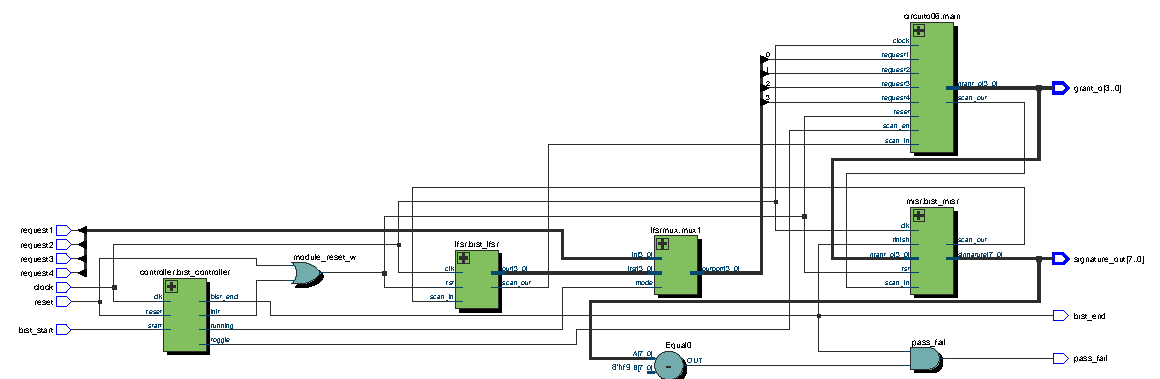
\includegraphics[scale=0.8]{block_diagram.pdf}
            \caption{Circular BIST block diagram.}
            \label{fig:bd}
    \end{figure}
    
\newpage
    
\section{Circular BIST testing and validation}

A multi-purpose testbech was created for the system's validation. 

A battery of tests included in the test-bench were used in order to check if the system is working is working properly and compliant to the given specifications . These tests are:

\begin{itemize}
  \item Single run, normal operation
  \item Multiple runs with reset sequence
  \item Multiple runs without reset sequence
  \item Mid start toggle
  \item Mid reset toggle
  \item Reset latch test
  \item Circuit operation with test vectors injection
\end{itemize}



The test to be run can be selected on the test-bench by setting the appropriate define condition. Only one test should be enabled at a time.

    \begin{lstlisting}[caption={Configurable test-bench parameters.},captionpos=b]
//VALIDATION TESTS
`define getfaultcoverage
// `define multiple_runs_reset
// `define multiple_runs
// `define mid_start
// `define mid_reset
// `define reset_latch
// `define vectest
    \end{lstlisting}  

    \subsubsection*{Circuit operation with test vectors injection}

The first test was to run the system in normal mode and a set of vectors were injected in order to check if the circuit is still working properly when embedded onto the BIST system.
\newpage

    \begin{lstlisting}[caption={Normal operation output.},captionpos=b]
Current vector: 0101
Circuit output: 4
Current vector: 1011
Circuit output: 8
Current vector: 0110
Circuit output: 4
Current vector: 1100
Circuit output: 8
Current vector: 1101
Circuit output: 8
Current vector: 0001
Circuit output: 1
Current vector: 0001
Circuit output: 1
Current vector: 1110
Circuit output: 8
Current vector: 0111
Circuit output: 4
Current vector: 0010
Circuit output: 2
    \end{lstlisting}  
    
    \subsubsection*{Single run, normal operation}
    
After this a single run in BIST mode was made to check the final signature in a perfect setup without faults. In our case the final signature is F9 (in hexadecimal format). This signature was updated on the design and another test was made in order to check if the ''pass\textunderscore fail'' signal was working as expected.

    \begin{lstlisting}[caption={BIST normal operation output.},captionpos=b]
Output signature: f9
Pass/fail: 1
    \end{lstlisting}  
 






    
    \subsubsection*{Multiple runs with reset sequence}
    
    On this test, the circuit must perform two runs with a reset sequence in between. The both BIST runs must end with the same result, F9 signature and ''pass\textunderscore signal'' indicating ''pass''.
    
    \begin{lstlisting}[caption={Multiple runs with reset sequence output.},captionpos=b]
linuxdev@linuxdev-VirtualBox:/media/sf_GitHub/PTFSE-Classes/Project2$ make circular_bist_test
Output signature: f9
Pass/fail: 1
Output signature: f9
Pass/fail: 1
    \end{lstlisting} 
    
    \subsubsection*{Multiple runs without reset sequence}
    
    Like before, on this test, the circuit must perform two consecutive runs but without a reset sequence in between. The both BIST runs must end with the same result, F9 signature and ''pass\textunderscore signal'' indicating ''pass''.
    
    \begin{lstlisting}[caption={Multiple runs without reset sequence output.},captionpos=b]
linuxdev@linuxdev-VirtualBox:/media/sf_GitHub/PTFSE-Classes/Project2$ make circular_bist_test
Output signature: f9
Pass/fail: 1
Output signature: f9
Pass/fail: 1
    \end{lstlisting}
    
    \subsubsection*{Mid reset toggle}
    
    On this test, the global reset signal is toggle during the BIST operation. In this case the module should stop operation and return to the default state.
    
    \subsubsection*{Mid start toggle}
    
    On this test, the start signal is toggle during the BIST operation. In this case the module should not affect the current operation.
    
    \subsubsection*{Reset Latch test}
    
    This test is used to check for proper operation of the reset latch. This test ensures that when start signal is sampled whilst the reset signal is on, the controller must wait for both the signals to go low and should only start on the next start signal if the reset signal is not enabled.

    
    
    \section{Synthesis}
    
    Once the circuit was fully tested, the top module was synthesized into one single module. The synthesized circuit was tested locally, and apart from some issues related with the tool-chain used (icarus + gtkwave), the circuit worked as intended. \\
    Full synthesis reports are present alongside this document with the project files.\\
    Synthesis reports were extracted for the original circuit and for the complete top module. Some comparisons can be made:
    
    \subsubsection*{Gate count and circuit area}
    
Report for the original circuit:

\begin{lstlisting}[caption={Gate count and circuit area of the given circuit.},captionpos=b]
  Gate   Instances    Area          Library      
-------------------------------------------------
AOI211           2    145.600    c35_CORELIB_TYP 
AOI2111          2    182.000    c35_CORELIB_TYP 
AOI221           9    819.000    c35_CORELIB_TYP 
CLKIN3           4    145.600    c35_CORELIB_TYP 
DFC3            13   4022.200    c35_CORELIB_TYP 
DFEC1           12   4149.600    c35_CORELIB_TYP 
IMUX20           1     91.000    c35_CORELIB_TYP 
IMUX21           1     91.000    c35_CORELIB_TYP 
INV0             1     36.400    c35_CORELIB_TYP 
INV2             2     72.800    c35_CORELIB_TYP 
INV3             1     36.400    c35_CORELIB_TYP 
NAND22           5    273.000    c35_CORELIB_TYP 
NAND31           1     72.800    c35_CORELIB_TYP 
NOR21            5    273.000    c35_CORELIB_TYP 
NOR31            7    509.600    c35_CORELIB_TYP 
NOR40            1     72.800    c35_CORELIB_TYP 
OAI2111          1     91.000    c35_CORELIB_TYP 
OAI212           9    655.200    c35_CORELIB_TYP 
OAI311           1     91.000    c35_CORELIB_TYP 
TFC3             1    291.200    c35_CORELIB_TYP 
-------------------------------------------------
total           79  12121.200                    
                                      
   Type    Instances    Area   Area % 
--------------------------------------
sequential        26  8463.000   69.8 
inverter           8   291.200    2.4 
logic             45  3367.000   27.8 
--------------------------------------
total             79 12121.200  100.0 
    \end{lstlisting} 
    
And for the full top module:
    
\begin{lstlisting}[caption={Gate count and circuit area of the full BIST system.},captionpos=b]
  Gate   Instances    Area          Library      
-------------------------------------------------
ADD22            6    873.600    c35_CORELIB_TYP 
AOI211           1     72.800    c35_CORELIB_TYP 
AOI2111          3    273.000    c35_CORELIB_TYP 
AOI221           4    364.000    c35_CORELIB_TYP 
AOI311           2    182.000    c35_CORELIB_TYP 
CLKIN2           2     72.800    c35_CORELIB_TYP 
CLKIN3           2     72.800    c35_CORELIB_TYP 
DF3             27   7371.000    c35_CORELIB_TYP 
DFS1             1    364.000    c35_CORELIB_TYP 
DFSC1           13   4968.600    c35_CORELIB_TYP 
DFSEC1          12   5241.600    c35_CORELIB_TYP 
IMUX20          23   2093.000    c35_CORELIB_TYP 
IMUX21           4    364.000    c35_CORELIB_TYP 
IMUX30           1    182.000    c35_CORELIB_TYP 
INV2            18    655.200    c35_CORELIB_TYP 
INV3             9    327.600    c35_CORELIB_TYP 
MUX22            5    546.000    c35_CORELIB_TYP 
NAND22          27   1474.200    c35_CORELIB_TYP 
NAND30           1     72.800    c35_CORELIB_TYP 
NAND31           4    291.200    c35_CORELIB_TYP 
NAND40           1     91.000    c35_CORELIB_TYP 
NOR20            1     54.600    c35_CORELIB_TYP 
NOR21           22   1201.200    c35_CORELIB_TYP 
NOR31           11    800.800    c35_CORELIB_TYP 
NOR40            4    291.200    c35_CORELIB_TYP 
OAI211           2    145.600    c35_CORELIB_TYP 
OAI2111          4    364.000    c35_CORELIB_TYP 
OAI212           5    364.000    c35_CORELIB_TYP 
OAI222           6    546.000    c35_CORELIB_TYP 
OAI311           1     91.000    c35_CORELIB_TYP 
TFSC1            1    345.800    c35_CORELIB_TYP 
XNR21            2    218.400    c35_CORELIB_TYP 
XNR31            1    200.200    c35_CORELIB_TYP 
XOR31            3    600.600    c35_CORELIB_TYP 
-------------------------------------------------
total          229  31176.600                    

   Type    Instances    Area   Area % 
--------------------------------------
sequential        54 18291.000   58.7 
inverter          31  1128.400    3.6 
logic            144 11757.200   37.7 
--------------------------------------
total            229 31176.600  100.0 
    \end{lstlisting} 
    
That make out an increase of $157.21\%$. 

After the circuit was successfully synthesised, the fault simulator was used to check for the current fault detection coverage:

\begin{lstlisting}[caption={Fault simulator results.},captionpos=b]
Stuck-At (0/1) Fault Table
			 Total #	 Prime #
Untestable		      0		      0
Detected		    344		    344
Potentially_detected	      7		      7
Undetected		     36		     36
Unobserved_detected	      0		      0
Unobserved_undetected	      0		      0
Dangerous_detected	      0		      0
Dangerous_undetected	      0		      0
Not_simulatable		    173		    173
Not_injected		     32		     32
Total			    592		    592
    \end{lstlisting} 
    
Using the following formula, it is possible to compute the fault coverage:
\begin{equation}
    \frac{\text{Detected}+ \text{Potentially detected}}{\text{Detected}+ \text{Potentially detected} + \text{Undetected}}\times 100 = \frac{344+7}{344+7+36}\times 100 = 90.7 \%        
\end{equation}   
    
With this we can confirm that the developed system achieves the required 90\% fault coverage.
    
 \newpage   
	
	\section{Conclusion}
	This project objective was to learn how to program and develop a Circular BIST to a given circuit which could also work with the controller developed for the first project of this course.\\
	Several tests were performed to the system and its modules, and corrections were made to the controller to guarantee this system works as it was intended to.\\
	The fault coverage surpasses the minimum requirement of 90\%.\\
	Most of the difficulties of this project landed upon a simulation difference between the toolchains used, icarus vs cadence. The system that was proven to be working locally did not work after it was synthesized. Our team spent a large amount of time in order to track down the issue which led us to have not much time left to improve the performance of the system. But overall, the developed system worked as expected and accomplishes all of the requirement set by the teacher.




\begin{thebibliography}{20}
\bibitem{ref1}
Verilog Tutorial (Course slides)\\
\url{https://fenix.tecnico.ulisboa.pt/downloadFile/1126518382240212/My%20Verilog%20Tutorial.pdf}

\bibitem{ref2}
Xillinx LFSR maximum length polynomial table\\
\url{https://www.xilinx.com/support/documentation/application_notes/xapp052.pdf}



\end{thebibliography}


% \appendix

% \section{Fa}

\end{document}
